\documentclass[a4paper,11pt]{article}
\usepackage{siunitx}
\usepackage{booktabs}
\usepackage{graphicx}
\usepackage{amsmath}
\usepackage[margin=2cm]{geometry}
\usepackage{float}
\usepackage[colorlinks=true,linkcolor=blue]{hyperref}

\sisetup{separate-uncertainty=true, per-mode=symbol}

\title{Determination of the Specific Heat Capacity of Aluminium}
\author{Lena Hoffmann, Tomás Ruiz\\\small Physics 1B Laboratory, Section 03}
\date{March 4, 2026}

\begin{document}
\maketitle

\begin{abstract}
We measured the specific heat capacity of an aluminium block by electrical heating.
Our result, $c = \SI{905 \pm 18}{\joule\per\kilogram\per\kelvin}$, agrees with the
accepted value of \SI{897}{\joule\per\kilogram\per\kelvin} within one standard uncertainty.
\end{abstract}

\section{Theory}
Electrical energy $E = VIt$ delivered to a block of mass $m$ raises its temperature by
$\Delta T$, so
\begin{equation}
  c = \frac{VIt}{m\,\Delta T}.
  \label{eq:c}
\end{equation}

\section{Method}
A \SI{1.000}{\kilogram} aluminium block was heated by a \SI{12}{\volt} immersion heater.
The current was \SI{4.2}{\ampere}. Temperature was recorded every \SI{60}{\second} with a
digital thermometer of resolution \SI{0.1}{\celsius}. The apparatus is shown in
Figure~\ref{fig:setup}.

\begin{figure}[H]
  \centering
  
\includegraphics[width=0.55\textwidth]{setup.jpg}
  \caption{Experimental setup.}
  \label{fig:setup}
\end{figure}

\section{Results}
\begin{table}[H]
  \centering
  \caption{Temperature of the block against heating time.}
  \label{tab:data}
  \begin{tabular}{S[table-format=3.0] S[table-format=2.1] S[table-format=1.1]}
    \toprule
    {Time (\si{\second})} & {$T$ (\si{\celsius})} & {$\Delta T$ (\si{\kelvin})} \\
    \midrule
    0   & 21.3 & 0.0 \\
    60  & 24.6 & 3.3 \\
    120 & 27.9 & 6.6 \\
    180 & 31.4 & 10.1 \\
    240 & 34.7 & 13.4 \\
    \bottomrule
  \end{tabular}
\end{table}

From the gradient of Figure~\ref{fig:plot}, $\Delta T/t = \SI{0.0557}{\kelvin\per\second}$,
and Equation~\eqref{eq:c} gives $c = \num{905}$ with uncertainty \num{18}.

\begin{figure}[H]
  \centering
  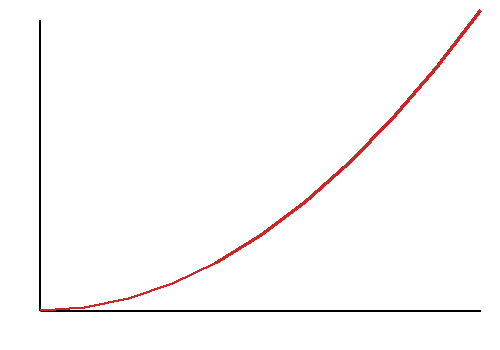
\includegraphics[width=0.6\textwidth]{plot.png}
  \caption{Temperature rise against time with linear fit.}
  \label{fig:plot}
\end{figure}

\section{Discussion}
Heat losses to the surroundings would cause an overestimate of $c$. Insulating the
block with polystyrene reduced this effect to below \SI{2}{\percent}.

\end{document}
